\documentclass[12pt]{article}
\usepackage[utf8]{inputenc}
\usepackage[russian]{babel}
\usepackage[left=1.5cm,right=1.5cm,top=1.5cm,bottom=2cm]{geometry}
\usepackage{graphicx}
\usepackage{color}
\usepackage{titlesec}
\usepackage{amssymb}
\usepackage{mathtools}
\usepackage{minted}
\usepackage{hyperref}
\usepackage{amsmath}
\usepackage{amsfonts}
\usepackage{fancyhdr}
\usepackage{enumitem}
\usepackage{mathbbol}
\usepackage{titlesec}
\usepackage{changepage}
\usepackage{listings}
\usepackage[titles]{tocloft}
\usepackage{tcolorbox}
\usepackage{tikz}
\usepackage{tikz-cd}
\usepackage{ulem}
\usepackage{nicefrac}
\usepackage{indentfirst}
\usepackage{dsfont}
\usepackage{csquotes}

\usepackage{hyperref}
\hypersetup{
    colorlinks=true,
    linkcolor=cyan,
    filecolor=magenta,      
    urlcolor=blue,
    pdftitle={Overleaf Example},
    pdfpagemode=FullScreen,
    }
\newcommand\nn{$\mathds{N}$}
\graphicspath{ {.} }
\title{\textbf{An Introduction to Mathematics of Financial Derivatives}}
\author{Григорий Злотин и Валерий Бигаев}
\date{...}
\begin{document}
\section{О целях работы}{
Главной целью работы было рассмотреть некоторые деривативные стратегии, посмотреть на их результаты на реальных данных, сравнить их результаты с стратегией Buy-and-hold, и отсюда сделать вывод о целесообразности их применения при формировании инвестиционного портфеля. 
\section{Введение}
Часто частные инвесторы считают, что на финансовых рынках вероятность того, что цена актива вырастет в рамках какого-то конкретного временного промежутка сильно зависит от динамики цены этого актива в прошлых временных промежутках.\par В нашем исследовании мы проверим, насколько разумно это предположение, чтобы решить, имеет ли смысл ориентироваться на прошлые цены акций при формировании портфеля. \\
\section{Разведочный анализ данных}
Датасеты взяты с Yahoofinance, мы брали данные по акциям из индекса FAANG(мы выбрали именно эти акции, так как они наиболее ликвидные, в них минимальные спреды, и соответственно мы можем считать, что наша заявка в любой момент будет исполнена по рыночной цене, а это достаточно важно при анализе цен акций).\\ \par
Очевидно, нам интересно предсказывать цену закрытия из имеющихся данных. При этом у нас есть параметры Open, Volume, High, Low.\\ \par
Проблема предсказания цены закрытия по параметрам Volume, High, Low очевидна: Эти параметры известны нам только в момент закрытия, а соответственно использовать их при предсказании мы не можем. Значит остается только предсказывать цену Close по цене Open. \\
В такой ситуации построение матрицы корреляций лишено смысла, так как мы буквально хотим предсказывать значение одной переменной, по значению другой.
\section{Модели}
\subsection{Простая бинарная классификация}
Для начала попробуем использовать методы классификации, такие как Классификатор дерева решений(\url{https://scikit-learn.ru/1-10-decision-trees/}), Логистическая регрессия(\url{https://habr.com/ru/companies/io/articles/265007/}) и метод k ближайших соседей(\url{https://habr.com/ru/articles/149693/})\\
\par
Все это - модели обучения с учителем, в которых мы сначала разбиваем выборку на обучающую и тестовую, размечаем данные в обучающей выборке и обучаем модель на них, а потом классифицируем объекты в тестовой.\\
\par Логистическая регрессия делит пространство объектов гиперплоскостью на две части(исходя из обучающей выборки), а потом исходя из границ этой гиперплоскости предсказывает классы объектов из тестовой выборки.
\\ \par
Метод k ближайших соседей предсказывает класс объекта исходя их классов ближайших к нему объектов(которые уже были классифицированы). Обычно берется евклидово расстояние.
\\ \par
Дерево решений является линейным классификатором, который выводит некоторый набор линейных правил на обучающей выборке(делит исходное множество гиперплоскостями), исходя из которых он делит данные на разные классы уже в тестовой выборке. 
\\
\\
Теперь, можем приступить непосредственно к задаче:
\\
\par
У нас есть датасет в котором есть цены открытия и закрытия данной акции(дневной таймфрейм). Каждый день мы можем классифицировать как "удачный"(Если цена закрытия больше цены открытия), или как "неудачный"(цена закрытия меньше цены открытия).\\ \par Соответственно, последовательности дней по такому правилу можно сопоставить последовательность нулей и единиц(0 - удачный день, 1 - неудачный день), и попытаться предсказывать каким будет $i$  день, если мы знаем, какими были $k$ дней до него. В нашем случае мы выбрали $k = 60$. \\
Анализ производился на акциях из индекса FAANG(кроме Meta), начиная с 2000 года.\\ \par
Хорошей метрикой качества наших моделей будет показатель accuracy, так как для данных акций на промежутке в примерно 20 лет количество падающих дней, хоть и меньше количества растущих, но достаточно незначительно(для акций из индекса FAANG их соотношение было не больше чем $\frac{52}{48}$).\\
\par Показатель recall нам интересен меньше, так как в нашей ситуации любой правильный прогноз приносит нам примерно одинаковую прибыль, и любой неправильный прогноз приносит нам соразмерные убытки.(К примеру, если бы мы предсказывали, есть ли рак у пациента, или нет, то цена ошибки, когда мы сказали что рака нет, в ситуации когда он есть гораздо хуже, чем ошибка, когда мы сказали, что рак есть, а его на самом деле нет, и в такой модели мы бы делали акцент на recall для класса "больной болен раком")\\ \par
Проведем некоторую интерпертацию полученных нами результатов:\\ \par
Показатель accuracy каждой из моделей оказался примерно равен $0.5$, как в случае попытки предсказать повышение цены, так и в случае попытки предсказать ее понижение, причем его небольшие отклонения вверх вполне можно объяснить тем, что объектов одного класса немного больше, чем объектов второго.\\ \par
Соответсвенно результат нашей стратегии оказался таким же, как если бы мы просто подбрасывали правильную монету, и исходя из рисунка на выпавшей стороне говорили бы, какая будет цена акций завтра.\\ \par
Более того, в такой ситуации стратегия принесет отрицательный ожидаемый доход, так как процент верных прогнозов по данному классификатору будет $50\%$, с учетом того, что при такой стратегии наша торговля будет достаточно активной(покупать, если классификатор показывает, что цена пойдет вверх, иначе, продавать), то с учетом комиссии брокера инвестор уйдет в минус.
\\
Для большей наглядности можно посмотреть на график ROC кривой:
\centering
\includegraphics[width=0.9\textwidth]{ROC.png}
\\
Эта кривая показывает то, насколько наша классификация отличается от рандомной(чем выще лежит ROC-кривая, тем лучше классификатор), которая нарисована на этом графике синим цветом(да, ее действительно сложно заметить здесь)).

\subsection{Модель ARIMA}
\begin{displayquote}
 Интегрированная модель авторегрессии — скользящего среднего — модель и методология анализа временных рядов. Является расширением моделей ARMA для нестационарных временных рядов, которые можно сделать стационарными взятием разностей некоторого порядка от исходного временного ряда. Модель ARIMA $(p,d,q)$ означает, что разности временного ряда порядка $d$ подчиняются модели ARMA $(p,q)$.
\end{displayquote}

Для начала была выполнена калибровка гиперпараметров модели на дата-сете акций META. По этим графикам и различным критериям:


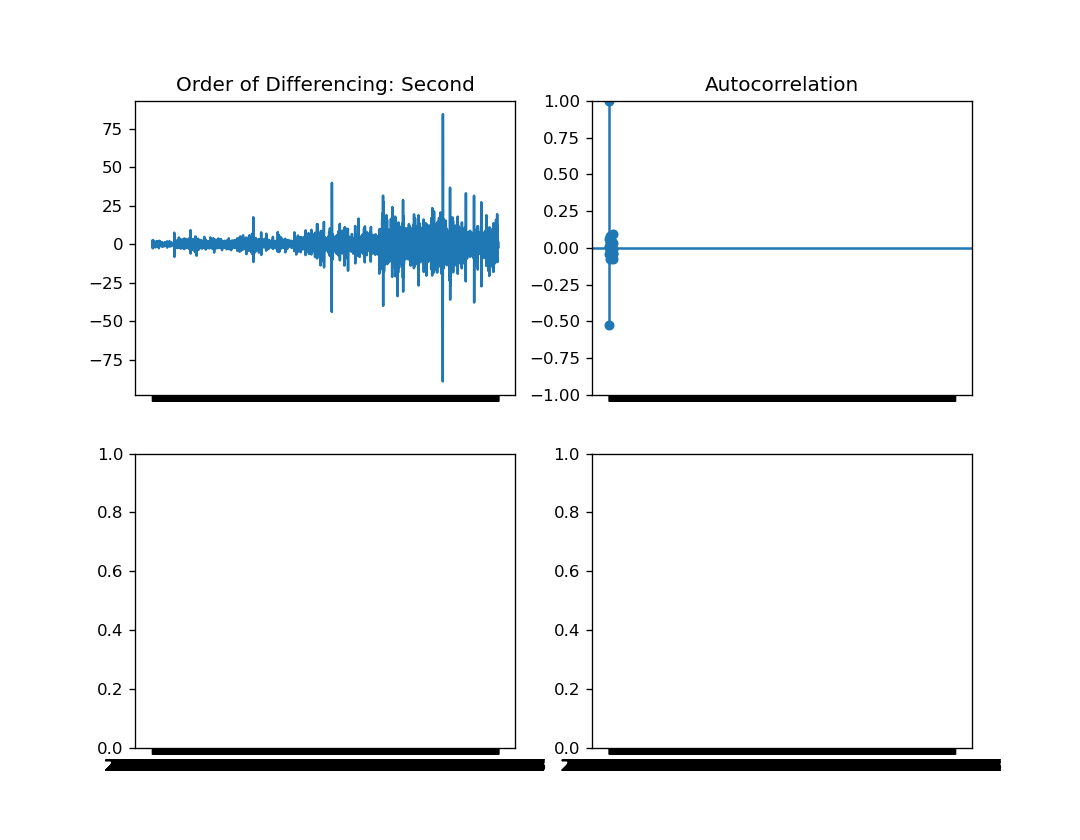
\includegraphics[width=0.9\textwidth]{Finding_d.png}

После калибровки было проведено тестирование модели по двум дата-сетам: акциям META и AAPL.

\begin{figure}[h]
\caption{META}
\centering
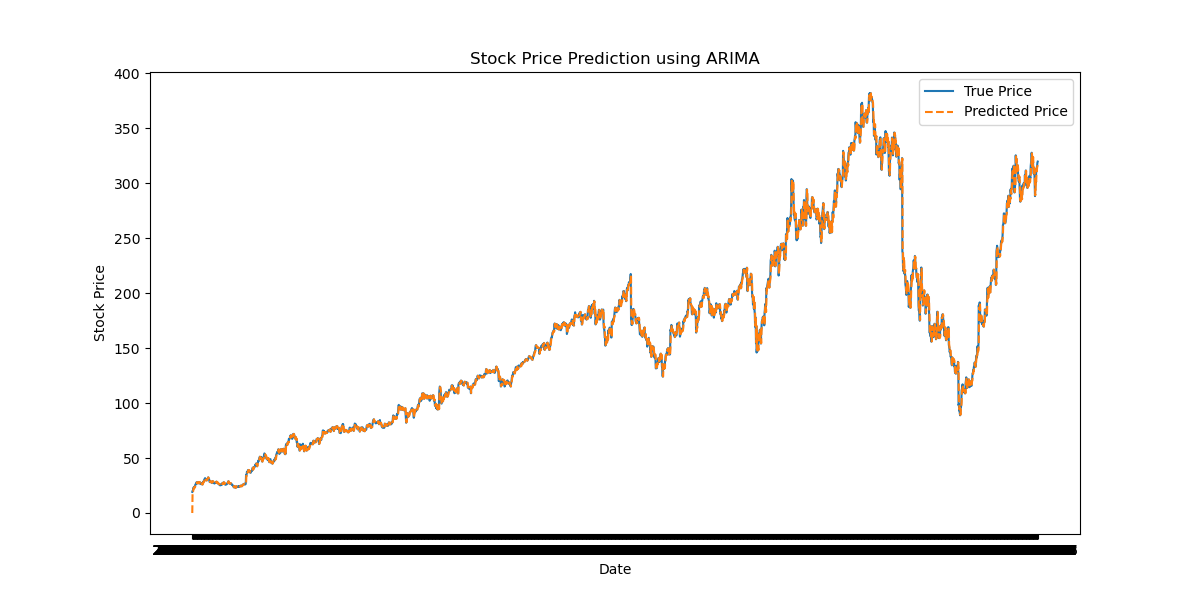
\includegraphics[width=0.9\textwidth]{ARIMA_META.png}
\end{figure}
\begin{figure}[H]
\caption{AAPL}
\centering
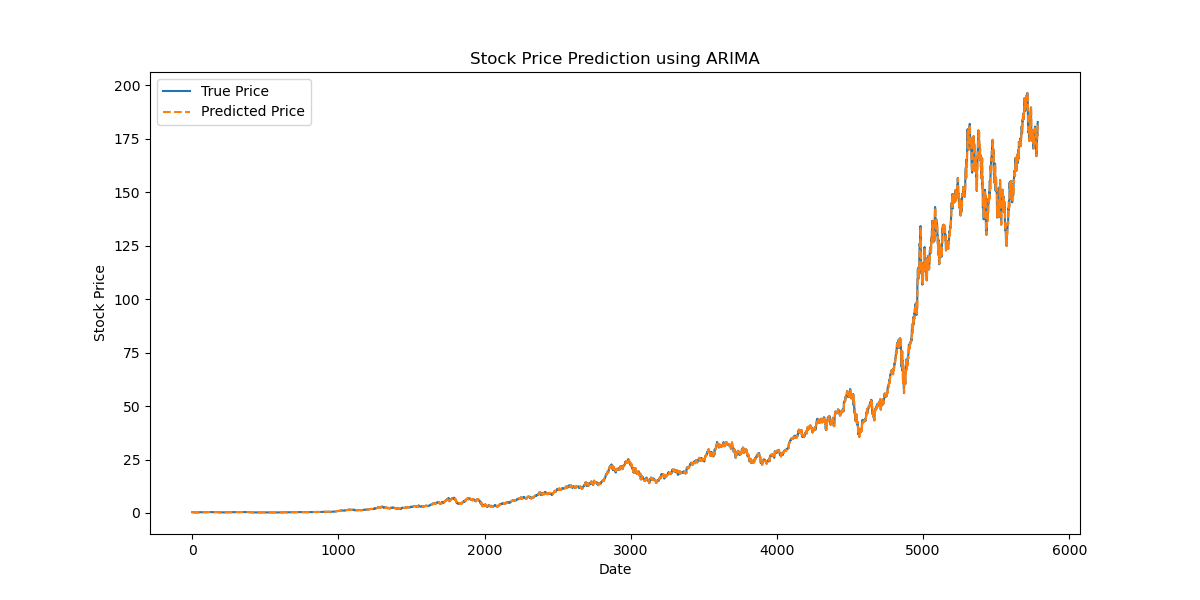
\includegraphics[width=0.9\textwidth]{ARIMA_AAPL.png}
\end{figure}

В частности на специально откалиброванном заранее дата-сете результаты были существенны (высокая прибыль), а на другом прибыль была достаточно мала(хоть она и была положительна, в сравнении с стратегий buy-and-hold она принесла меньший доход(Buy-and-Hold - примерно 100 долларов на акцию, ARIMA, с учетом всех комиссий - около 36 долларов на акцию)).
\\
\section{Вывод}
Частному инвестору при попытке выбирать акции для своего портфеля не стоит уделять много внимания прошлым ценам активов. Даже если акция находится в нисходящем тренде, вероятность вырасти в следующий день у нее будет такой же, как если бы она росла несколько недель подряд. \\
Также не стоит формировать свой инвестиционный портфель исходя из моделей, основанных на случайных процессах, которые анализируют только цены акций(возможно, добавление других переменных может улучшить результат, но это уже тема другого исследования(возможно, для финального проекта)).

\end{document}
